\chapter{Experimental Setting}
\label{chapter:Experimental Setting}

This chapter provides information about the experimental setting for the validation of the proposed method Batch Deep COACH (BD-COACH). Experiments are done both in simulation with a simulated teacher and in a real setup with a human teacher.


\section{Meta-World Benchmark}
\label{section:Meta-World Benchmark}
To evaluate BD-COACH and compare its performance to the base method D-COACH, we use three simulated environments from the open-source benchmark Meta-World \cite{metaworld}. Meta-World 
provides 50 standardized manipulation tasks that employ a simulated Sawyer robot arm. All Meta-World tasks are implemented in the MuJoCo physics engine \cite{mujoco}, and they are interfaced with OpenAI Gym \cite{openai} making these environments easy to use. Even if this benchmark was specifically designed for multi-task and meta-reinforcement learning, it is possible to simply access single goal environments as we do for this work. 
The three chosen tasks are plate-slide-v2, drawer-open-v2 and button-press-topdown-v2. There are several reasons behind the selection of these tasks. First, for each of them, Meta-World includes an oracle policy that commands the best action for the agent to take at every given time step. The usage of these policies as oracles allows running automated experiments easily, more information in Subsection \ref{subsection:Synthesised Feedback}. Secondly, these tasks use a manipulator similar to the real one that we have available and which we use for the validation in a real setup. Furthermore, from all the tasks that the benchmark provides, we choose three of them that do not involve opening and closing the gripper of the Sawyer's end effector. The reason behind this decision is that we focus on learning continuous actions, but the state of the gripper is either open or close. Finally, the three tasks are quite different between them, which allows generalizing the performance of BD-COACH.

All the tasks in Meta-World need an agent that executes an action in the environment equal to $[\delta x, \delta y, \delta z, g]$. The first three dimensions of the action correspond to the change in position of the end effector in the three Cartesian axes. The last dimension represents the gripper effort that keeps the fingers of the end effector open or close. In our case, for this dimension, the expert policy always commands a constant value keeping the gripper open or close depending on the task.
The observation space is a 9 dimensional space formed by the 3D Cartesian positions of the end effector, the object and the goal. In the case of the plate-slide-v2 task, the object refers to the puck, for the drawer-open-v2 task, the object is the handle and finally, in the task button-press-topdown-v2, the object is the button that can be moved vertically.

The Meta-World benchmark defines a success metric as the evaluation criterion for their tasks. This metric, ${\left\lVert \text{object}-\text{goal} \right\rVert}_2 < \epsilon$, is based on the euclidean distance between the object position and the goal position where $\epsilon$ is a small distance threshold that varies from task to task.

% Tambien diferenciamos entre experimentos que usan posiciones absolutas en la observacion, y experimentos que usan posiciones relativas.
% Primero realizamos


% Regarding the observation space we need to clearly differentiate between experiments where we use relative positions and experiments with absolute
% Relative positions versus absolute positions


\subsection{Simulated Experiments}
\label{subsection:simulated-experiments}


% After running some initial experiments, we observe that the way in which the observations are fed to the agent highly influence its performance. 
% If the positions are absolute, $[[xyz_\text{end effector}], [xyz_\text{object}], [xyz_\text{goal}]]$, tasks become harder specially for D-COACH.
% On the other hand, using relative position between the object and the end effector and the goal and the object, $[[xyz_\text{object} - xyz_\text{end effector}], [xyz_\text{goal} - xyz_\text{object}]]$, the number of dimensions decreases and, it is easier for the neural network to generalize the stages of the task. 


The goal of the simulated experiments is to compare the performance between BD-COACH and D-COACH as a function of the amount of data required to solve a task. To achieve this, we design an experiment where we first use states with relative positions and afterwards, we repeat the experiments changing to absolute positions. The reason behind this design choice is that states formed by relative positions, $ s= [[xyz_\text{end effector}], [xyz_\text{object}], [xyz_\text{goal}]]$, make it easier for the robot to generalize as the number of dimensions decreases. Furthermore, relative positions are more informative, and thus the model has to learn fewer correlations. On the other hand, states formed by absolute positions, $s = [[xyz_\text{object} - xyz_\text{end effector}], [xyz_\text{goal} - xyz_\text{object}]]$ make the task harder to learn as the number of dimensions increases.  

The simulated experiments are therefore divided into two phases. First, with observations formed by relative positions, different values of the parameters error magnitude, $e$, and replay buffer size, $K$, are tested to see how robust are BD-COACH and D-COACH to these variations. Specifically, we try three different values of $e$ and three values of $K$, each time fixing one of them and varying the other to see its effect. For the values of $e$, we chose 0.01, 0.1 and 1 as these values are within a range previously known to work. The three buffer sizes $K$ are 3000, 15000 and 30000; these sizes correspond to the 10\%, 50\% and 100\% respectively of the average accumulated corrections given by the simulated teacher at the end of the training. Once the previous experiments are done, we choose the best combination of parameters $e$ and $K$ for each method, and then the experiments are repeated with those same values but with observations formed by absolute positions. The parameters used for the policy and the human model are shown in Table \ref{tab:hyperparameters}. Trainings are 75000 time steps long which is approximately equivalent to 15 minutes of simulated time as the time step duration of the simulation is 0.0125 seconds.





\begin{table}[H]
\centering
\renewcommand{\arraystretch}{1.4}
\begin{tabular}{llS[table-format=2.2]SSS[table-format=2.2]S[table-format=2.2]}
\toprule
\textbf{Parameter }& \textbf{Value}\\[-.4em]
\midrule
Policy hidden layer sizes  &   (256, 128)\\
Policy activation of hidden layers  &   (tanh, tanh)\\
Policy learning rate  &  0.001\\
Human model hidden layer sizes &   (512, 512)\\
Human model activation of hidden layers  &   (tanh, tanh)\\
Human model learning rate  &   0.001\\
Buffer sampling rate&   10\\
Buffer sampling size &   20\\
\bottomrule
\end{tabular}
\caption{Parameters used for the simulated experiments}
\label{tab:hyperparameters}
\end{table}



\subsection{Task plate-slide-v2}
\label{subsection:metaworld-hockey-task}
The task plate-slide-v2, which resembles a hockey movement, can be seen in Figure \ref{fig:sequence-plate-slide}. The gripper of the end effector has to approach the puck, press it vertically and then slide the puck to the goal. If the puck goes inside the goal in less than 500 time steps, the episode is considered successful and a fail otherwise. The task starts with the gripper and the object always initiated at the same position whereas the goal is initiated randomly within an area of  $0.01m^2$. During all the episode the oracle commands the gripper to remain closed. The success metric that Meta-World defines for this task is ${\left\lVert \text{object}-\text{goal} \right\rVert}_2 < 0.07$.

 \begin{figure}[H]
  \centering
  \hspace*{\fill}%
  \subfloat[1 - Approach to puck]{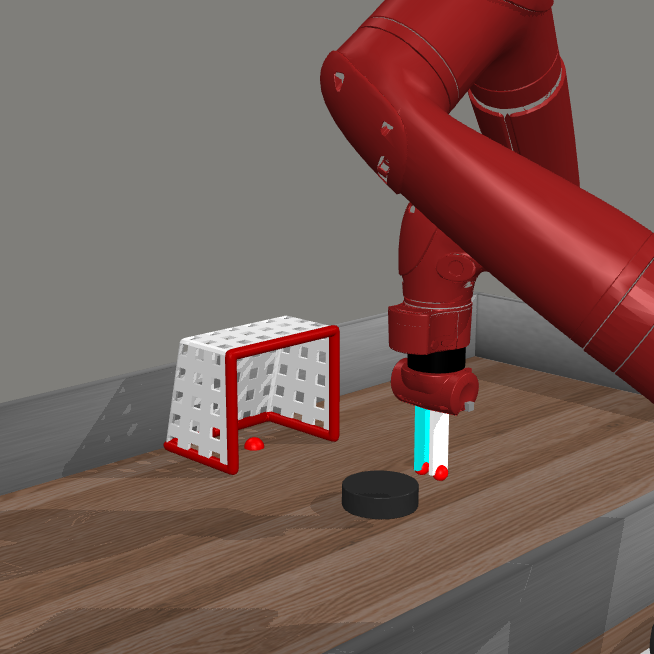
\includegraphics[width=0.23\textwidth]{figures/hockeypos0_v2.png}\label{fig:hockey_pos_0}}
   \hfill
  \subfloat[2 - Press puck vertically]{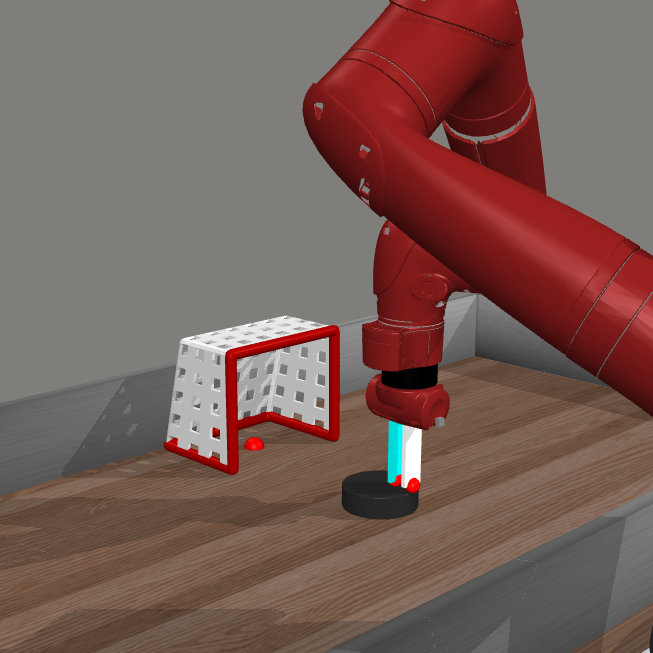
\includegraphics[width=0.23\textwidth]{figures/hockeypos1_v2.png}\label{fig:hockey_pos_1}}
   \hfill
  \subfloat[3 - Slide puck to goal]{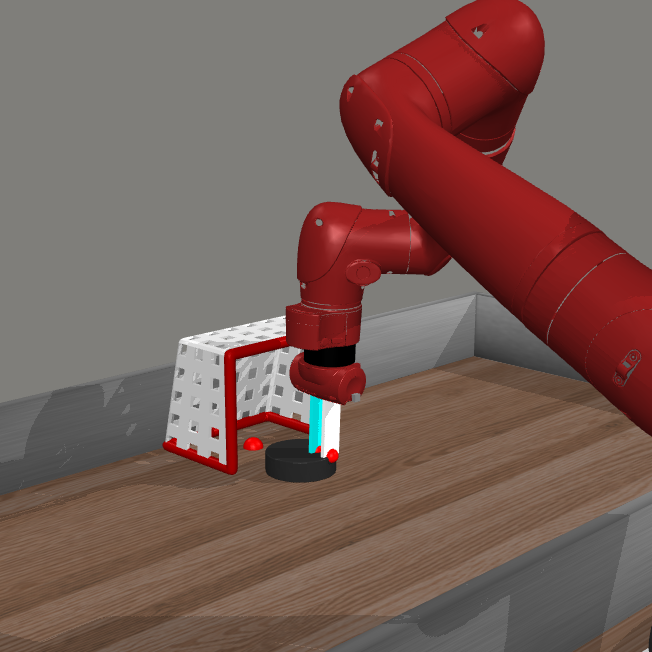
\includegraphics[width=0.23\textwidth]{figures/hockeypos2_v2.png}\label{fig:hockey_pos_2}}
  \hspace*{\fill}%
  \caption{Sequence of the plate-slide-v2 task in Meta-World}.
  \label{fig:sequence-plate-slide}
\end{figure}


\subsection{Task drawer-open-v2}
\label{subsection:metaworld-open-drawer-task}


The second simulated Meta-World task is called drawer-open-v2, see Figure \ref{fig:sequence-drawer}. For an episode to be considered a success, the end effector has to approach the handle of the drawer which is always initiated closed, hook to it and pull to open it in less that 500 time steps.
For this task, and following the oracle's command, the gripper remains open during all the episodes. The end effector is initiated always at the same position and the drawer can appear at a random position within a length of $0.2m$. The success metric for this task is ${\left\lVert \text{object}-\text{goal} \right\rVert}_2 < 0.03$.
 




 \begin{figure}[H]
  \centering
  \hspace*{\fill}%
  \subfloat[1 - Approach to handle]{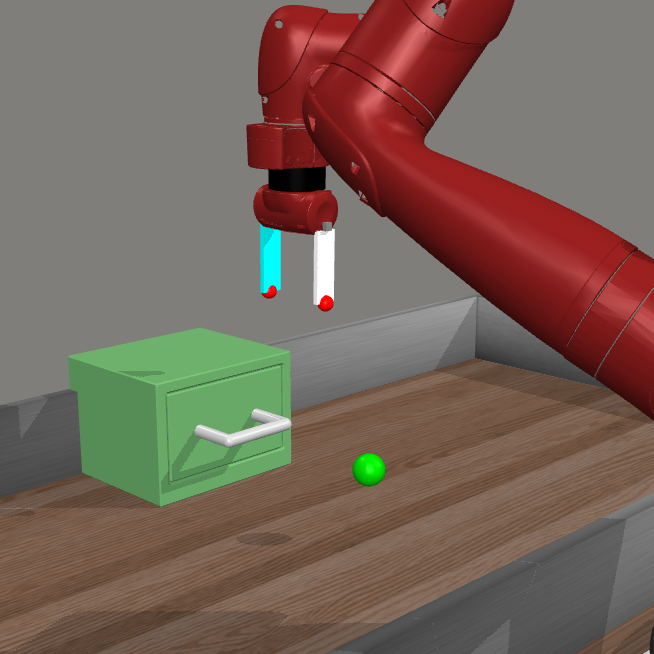
\includegraphics[width=0.23\textwidth]{figures/drawerpos0_v2.png}\label{fig:drawer_pos_0}}
   \hfill
  \subfloat[2 - Hook handle]{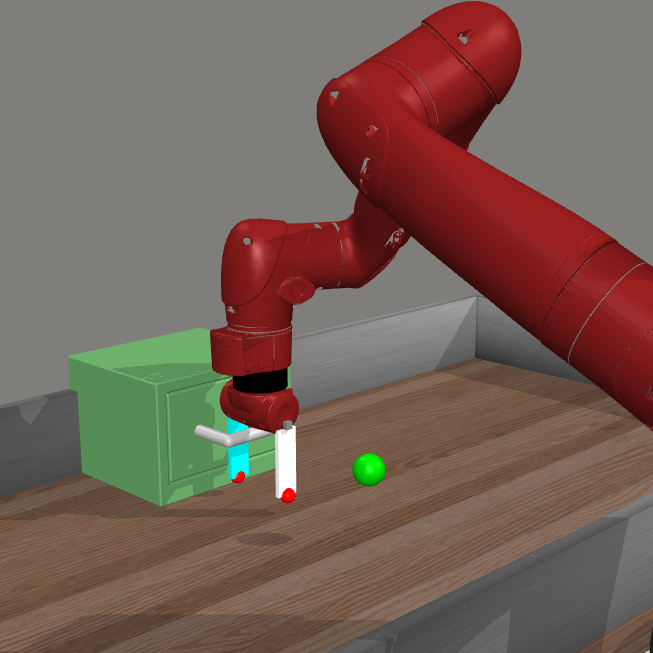
\includegraphics[width=0.23\textwidth]{figures/drawerpos1_v2.png}\label{fig:drawer_pos_1}}
   \hfill
  \subfloat[3 - Open drawer]{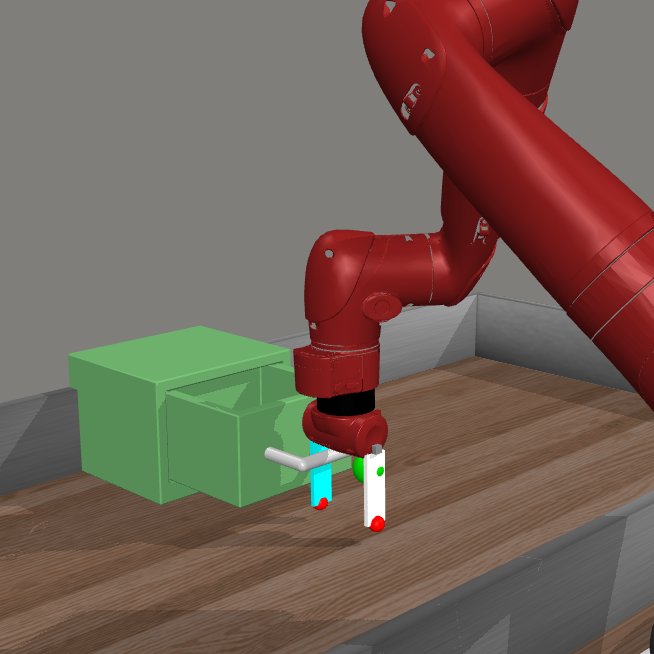
\includegraphics[width=0.23\textwidth]{figures/drawerpos2_v2.png}
  \label{fig:drawer_pos_2}}
  \hspace*{\fill}%
  \caption{Sequence of the drawer-open-v2 task in Meta-World}.
  \label{fig:sequence-drawer}
\end{figure}


\subsection{Task button-press-topdown-v2}
\label{subsection:metaworld-button-press-topdown-v2}

The final simulated Meta-World task is called button-press-topdown-v2, see Figure \ref{fig:sequence-button}. For an episode to be considered successful, the end effector has to reach the button, which is placed perpendicular to the surface of the table, and press it vertically in less that 500 time steps.
In this task, the gripper remains closed during all the episodes. The end effector is initiated always at the same position whereas the button is initiated randomly within an area of  $0.02m^2$. The success metric for this task is ${\left\lVert \text{object}-\text{goal} \right\rVert}_2 < 0.02$.

 \begin{figure}[H]
  \centering
  \hspace*{\fill}%
  \subfloat[1 - Approach to button]{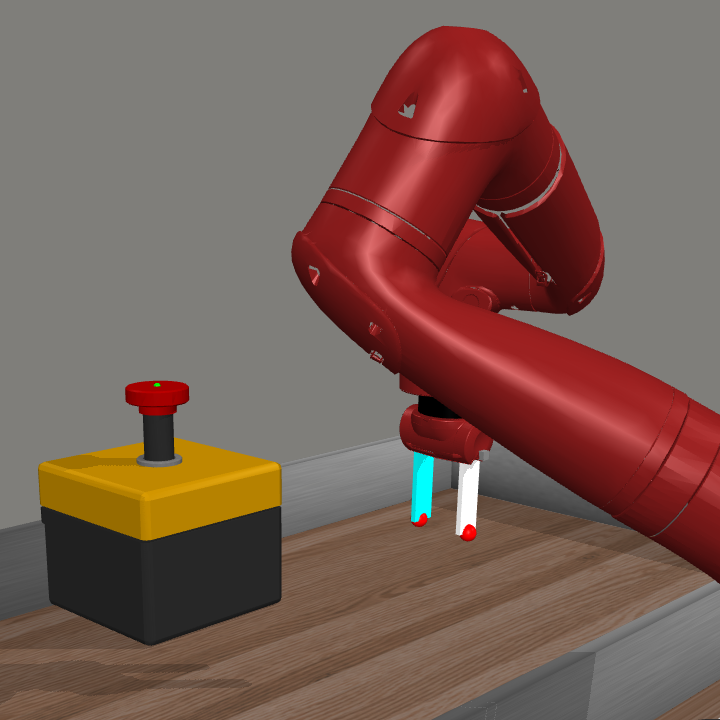
\includegraphics[width=0.23\textwidth]{figures/button_1.png}\label{fig:button_pos_0}}
   \hfill
  \subfloat[2 - Reach button]{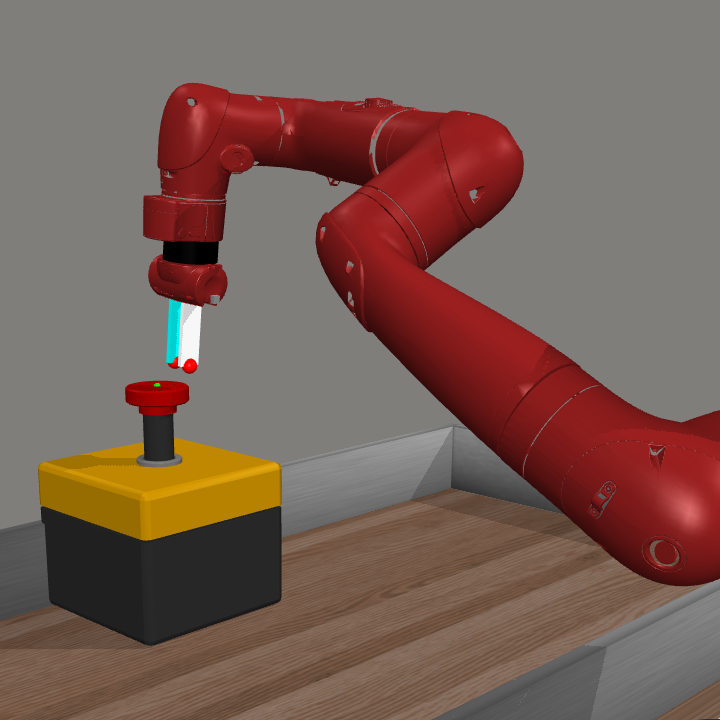
\includegraphics[width=0.23\textwidth]{figures/button_2.png}\label{fig:button_pos_1}}
   \hfill
  \subfloat[3 - Press button vertically]{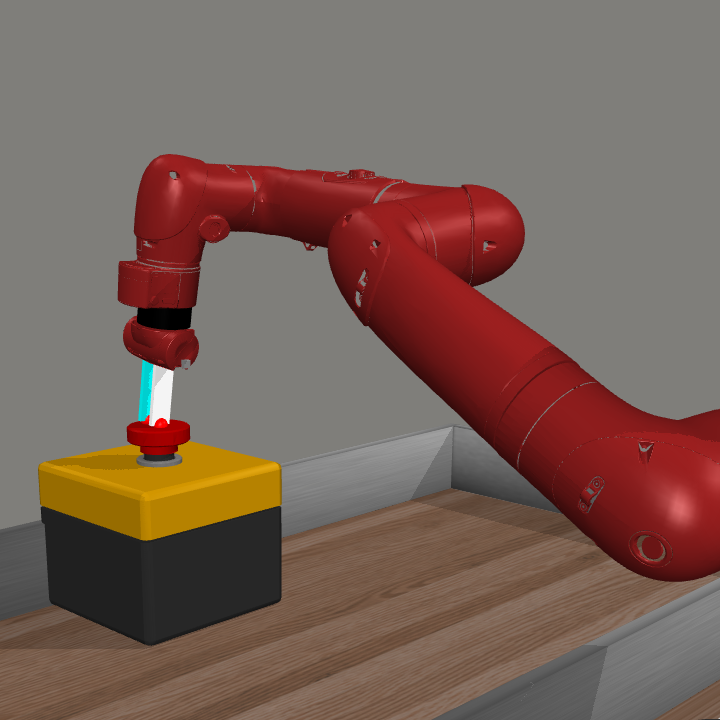
\includegraphics[width=0.23\textwidth]{figures/button_3.png}
  \label{fig:button_pos_2}}
  \hspace*{\fill}%
  \caption{Sequence of the button-press-topdown-v2 task in Meta-World}.
  \label{fig:sequence-button}
\end{figure}





\subsection{Synthesised Feedback}
\label{subsection:Synthesised Feedback}



For the simulated experiments, we employed an oracle or synthesized human teacher to provide feedback corrections. Using an oracle removes human factors such as the human teacher providing inconsistent feedback or he/she getting tired which would make comparisons between algorithms unfair. Furthermore, in order to compare performances of different frameworks, it is necessary to run many simulations to obtain a good average of the results which would be completely impractical if the teacher was a real human. Oracles can provide erroneous corrections to better simulate the behaviour of a person but in our case, the oracle gives always the best action for a particular state. 
For each of the three tasks explained before, we use the high-performance policies that the Meta-World benchmark provides for each of its tasks. The oracle used in this work generates feedback by computing $h = \operatorname{sign}(a_\text{teacher} - a_\text{agent})$, whereas the decision on whether to provide feedback at each time step is given by the probability $P_h = \alpha \cdot \operatorname{exp}(-\tau \cdot \operatorname{time step})$, where $\{\alpha \in \mathbb{R}\, | 0 \leq \alpha \leq 1 \}$; $\{\tau \in \mathbb{R} \, | 0 \leq \tau\}$. Furthermore, this binary feedback $h$ is only provided if the difference between the action of the policy and the action of the teacher is larger than a threshold $\epsilon$.





\section{Experiments with KUKA Robot Arm}
\label{section:Experiments with KUKA robot arm}

In order to validate the new proposed method BD-COACH on a real robotic setup with real human teachers, we devised two tasks involving a KUKA LBR iiwa 7 robot arm pushing a box placed on top of a table. These two tasks are explained in more detail in the following subsections. Several reflecting markers were attached to the box so its pose could be tracked by an OptiTrack motion capture system. The pose, captured by the eight cameras of the available OptiTrack system, consists of the position and orientation of the central point on the box created by the reflecting markers. The human that supervises the learning process conveys the corrections with a joystick. To make the task easier to teach, the human provides corrections just in the 2 axis parallel to the surface of the table while the vertical position of the end effector is kept constant and close to the surface of the table. Prior to performing the real experiments, everything was checked in a simulated Gazebo environment.

A ROS network connects all the required elements for the experiment, these being: The joystick with which corrections are sent, the information with the pose of the box from the OptiTrack and the position of the end effector of the KUKA robot. Specifically, for retrieving the position and sending the commands to the robot arm, the iiwa ROS stack \cite{iiwa} is used. For the control of the arm, we choose the \textit{CustomControllers} from the iiwa stack as it allows the control of the end effector in the Cartesian space. The control command is 6 dimensional where the first 3 values are the orientation of the end effector and the last 3 values are its position. For our purposes, we fix the orientation and the position in the vertical axis. The requested command in the remaining 2 positions is the current position of the end effector plus a delta which is the output of the network. Therefore, the policy outputs 2-dimensional actions representing the relative changes to the positions in the axes parallel to the table.

Regarding the observation that is fed to the policy, it is a 7-dimensional array whose components are: 1. The relative position between the end effector and the box in the x-axis (the axis parallel to the length of table), 2. The relative position between the end effector and the box in the z-axis (the axis parallel to the width of the table), 3. Velocity of the end effector in the x-axis, 4. Velocity of the end effector in the z-axis, 5. Position of the box in the x axis, 6. Position of the box in the z-axis, 7. Orientation of the box (the pitch angle perpendicular to the surface of the table). Finally, a simple metric of success is implemented. This metric has a value of 1 if the box ends within a small radius from the target position and 0 otherwise.

\subsection{Task kuka-push-box}
\label{subsection:Push box in a straight line}

For the first task called kuka-push-box, the KUKA arm has to push a box placed on one side of the table to a goal position indicated with a green cross. This task, that may seem trivial at first glance, is known as the \textit{pusher-slider system} \cite{constant_velocity} and it really highlights the importance of reactive robots. It is challenging because it involves an unstable system.
Pushing an box in a straight line without a reactive robot is simply impossible to achieve as the box will naturally fall outside the desired straight trajectory. Figure \ref{fig:planar-motion-problem} shows this problem where a constant velocity is commanded to the end effector but, because the robot does not react to the misalignments, the box keeps deviating from the desired straight trajectory.


 \begin{figure}[H]
  \centering
  \hspace*{\fill}%
  \subfloat{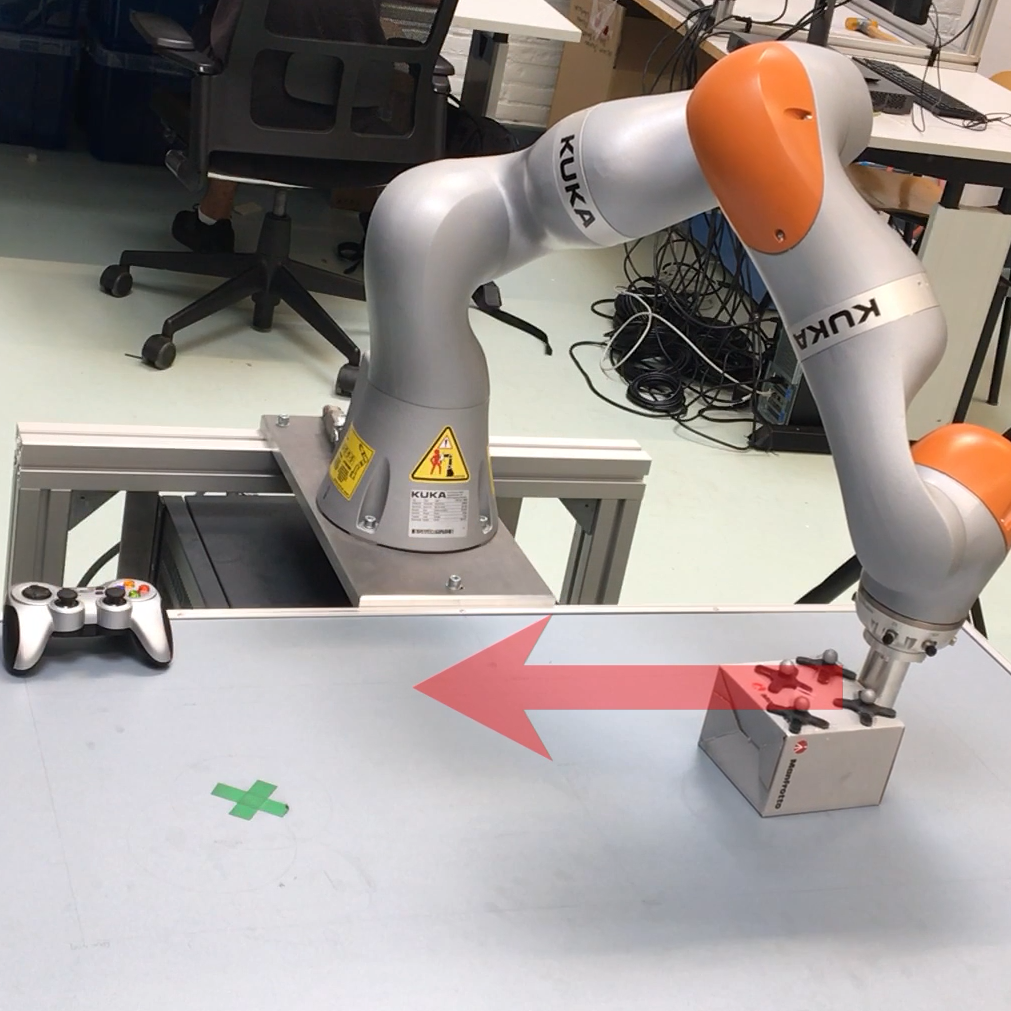
\includegraphics[width=0.22\textwidth]{figures/const_vel0.png}\label{fig:drawer_pos_0}}
   \hfill
  \subfloat{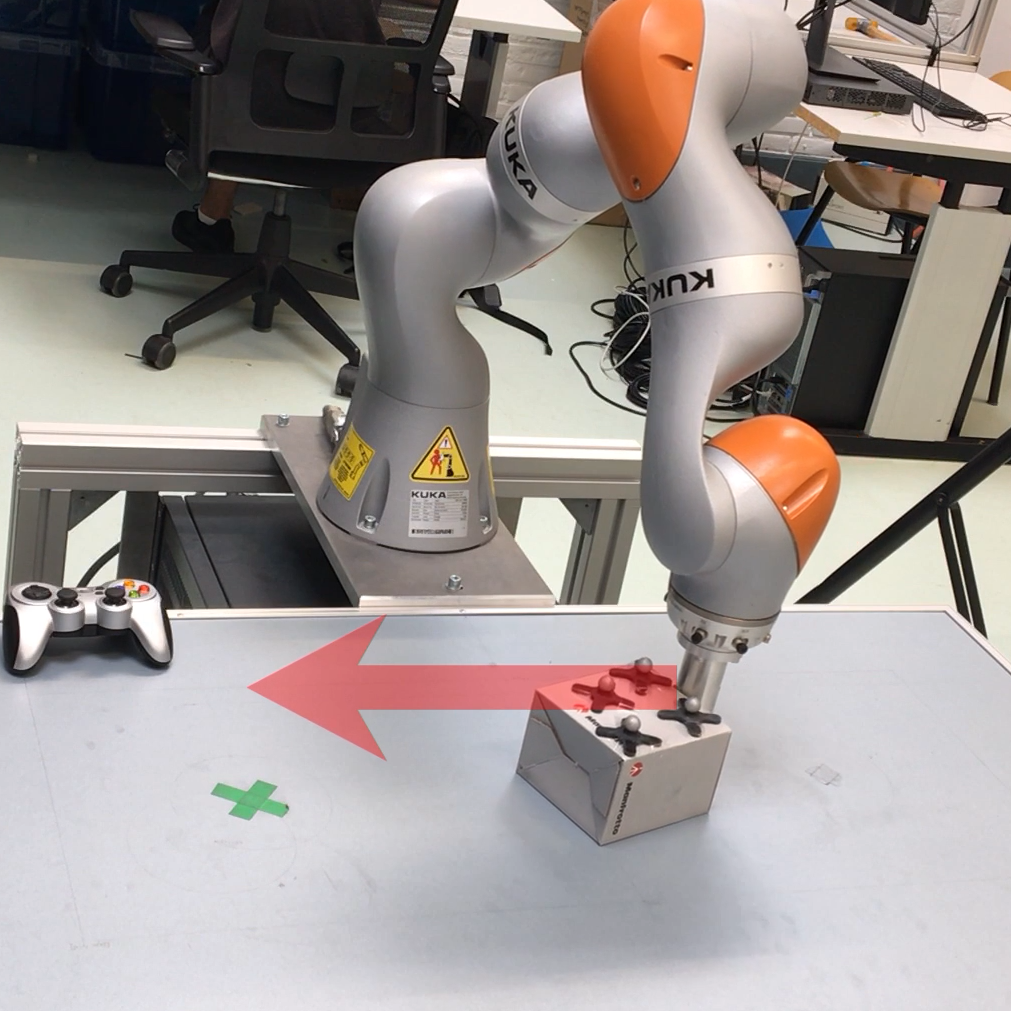
\includegraphics[width=0.22\textwidth]{figures/const_vel1.png}\label{fig:drawer_pos_1}}
   \hfill
  \subfloat{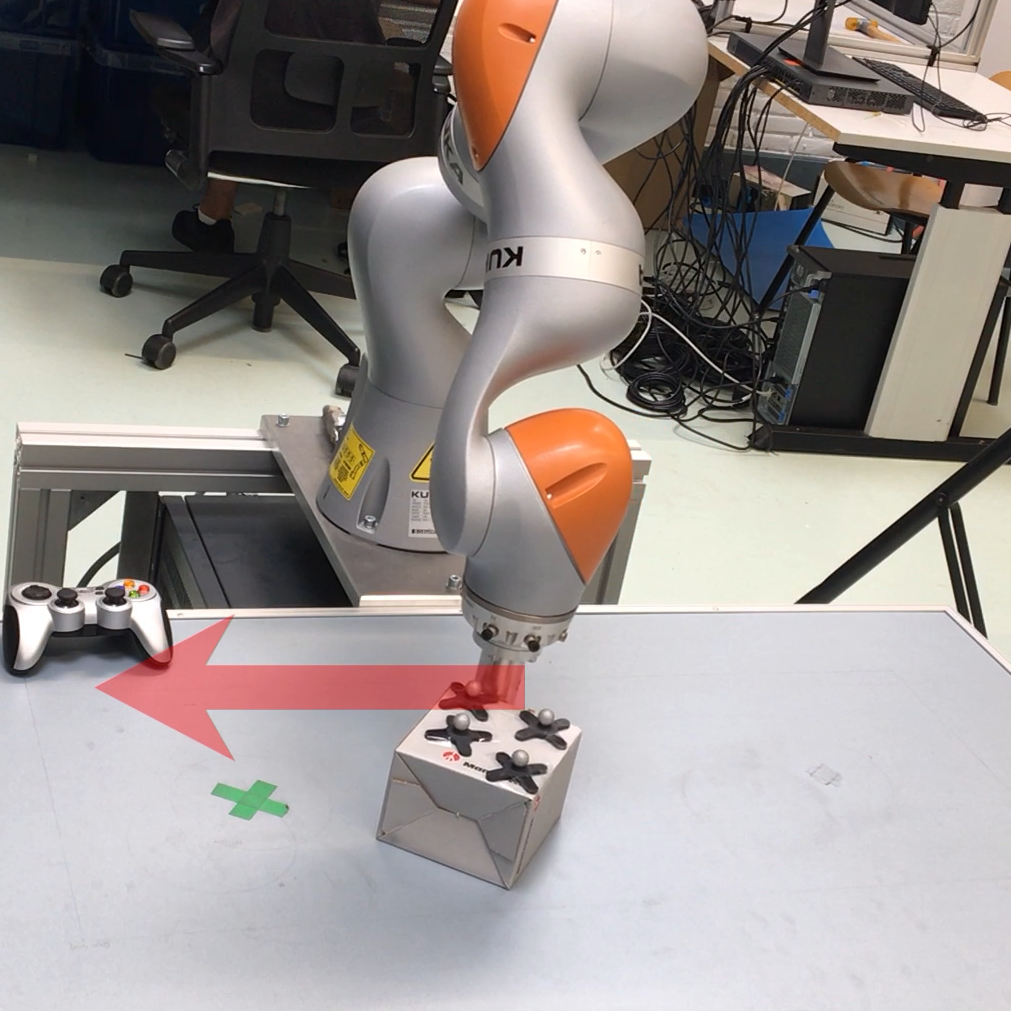
\includegraphics[width=0.22\textwidth]{figures/const_vel2.png}\label{fig:drawer_pos_2}}
   \hspace*{\fill}%
  \caption{By applying a constant velocity (red arrow), the box gets easily misaligned.}
  \label{fig:planar-motion-problem}
\end{figure}

Figure \ref{fig:sequence-push-box} shows a sequence of the task push-box once the BD-COACH has learnt it. The box is initialized at random positions and disturbances are manually introduced. The agent is able to successfully reach the goal by learning a continuous back and forth motion that makes it possible to quickly correct the misalignments of the box when it starts changing its orientation.

 \begin{figure}[H]
  \centering
  \subfloat[1 - Start position]{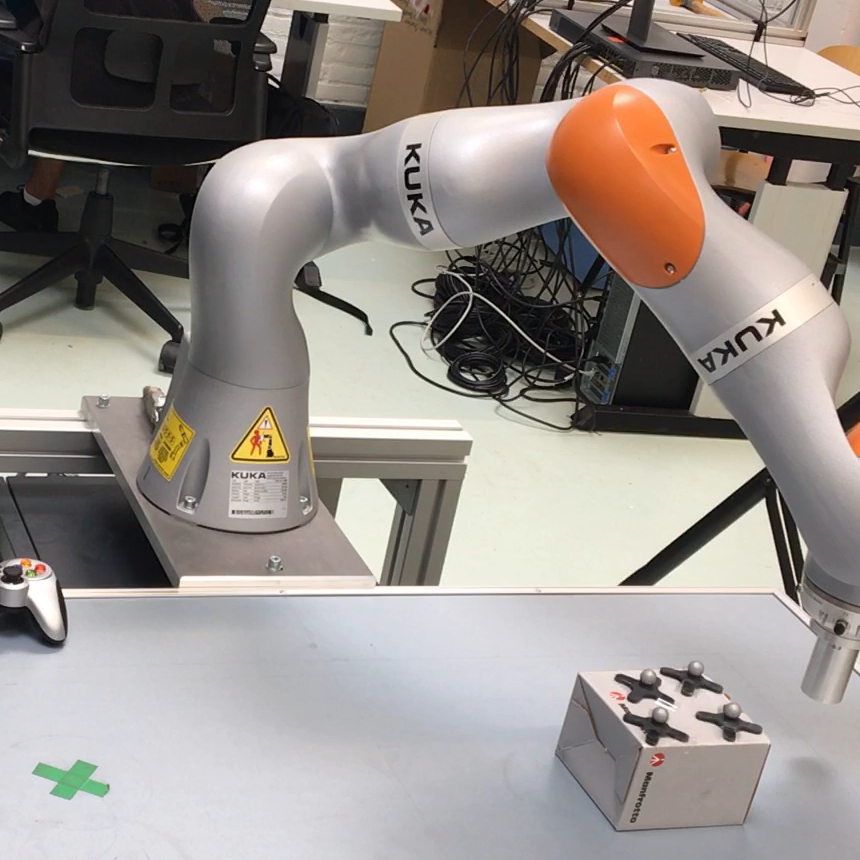
\includegraphics[width=0.19\textwidth]{figures/push0.png}\label{fig:push_pos_0}}
   \hfill
  \subfloat[2 - Approach to box]{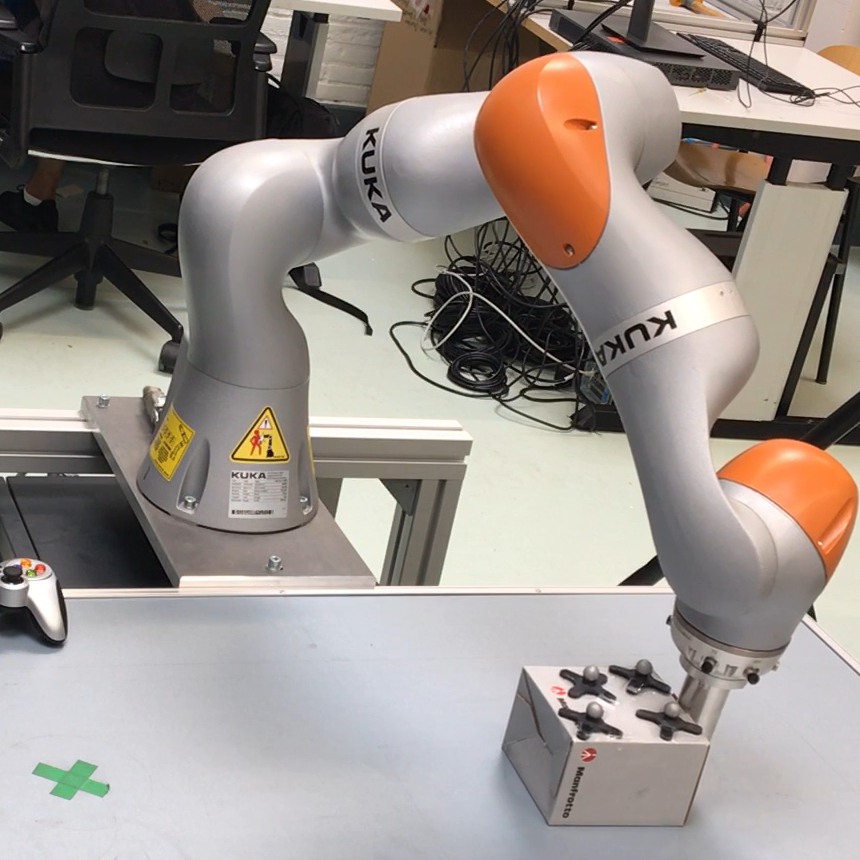
\includegraphics[width=0.19\textwidth]{figures/push1.png}\label{fig:push_pos_1}}
   \hfill
  \subfloat[3 - Introduce disturbance]{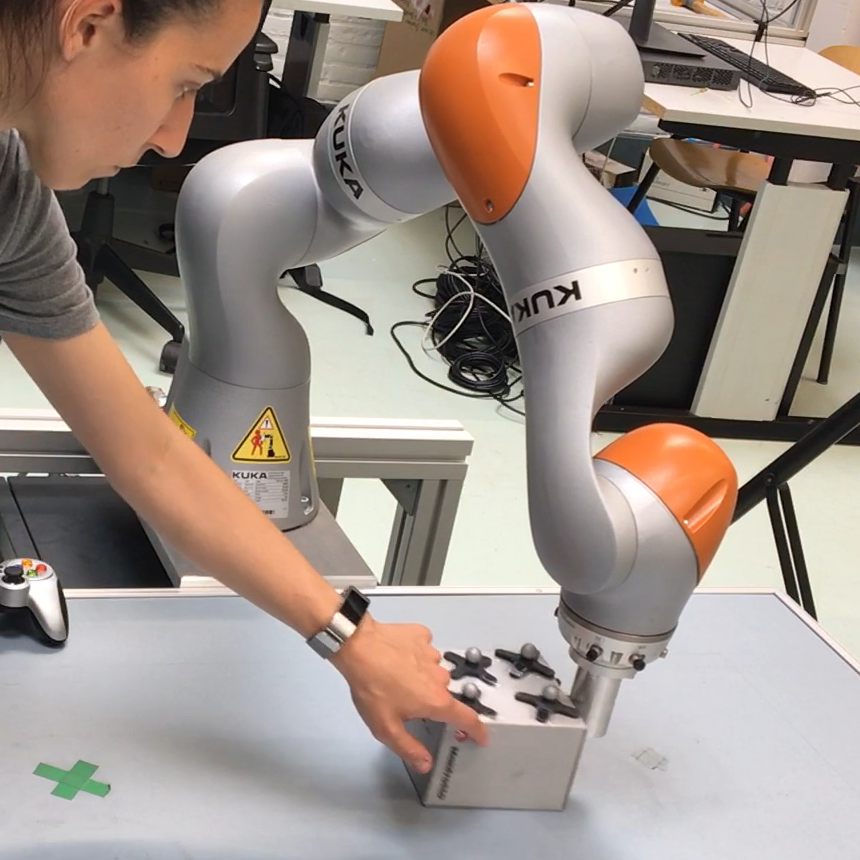
\includegraphics[width=0.19\textwidth]{figures/push2.png}\label{fig:push_pos_2}}
   \hfill
  \subfloat[4 - Correct disturbance]{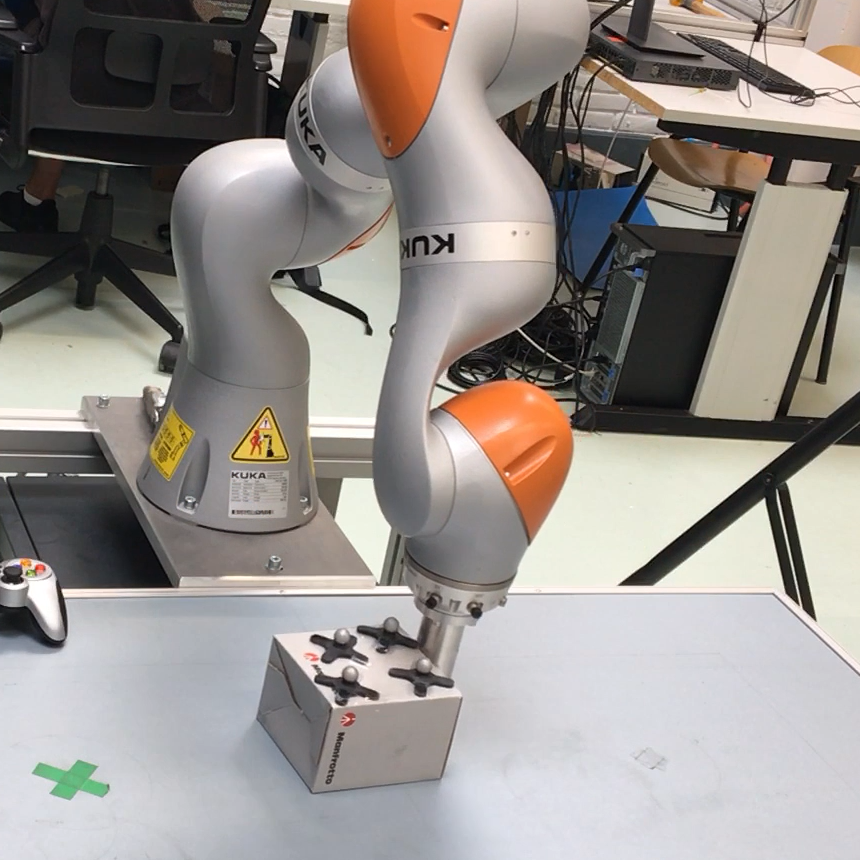
\includegraphics[width=0.19\textwidth]{figures/push3.png}\label{fig:push_pos_2}}
   \hfill
  \subfloat[5 - End position]{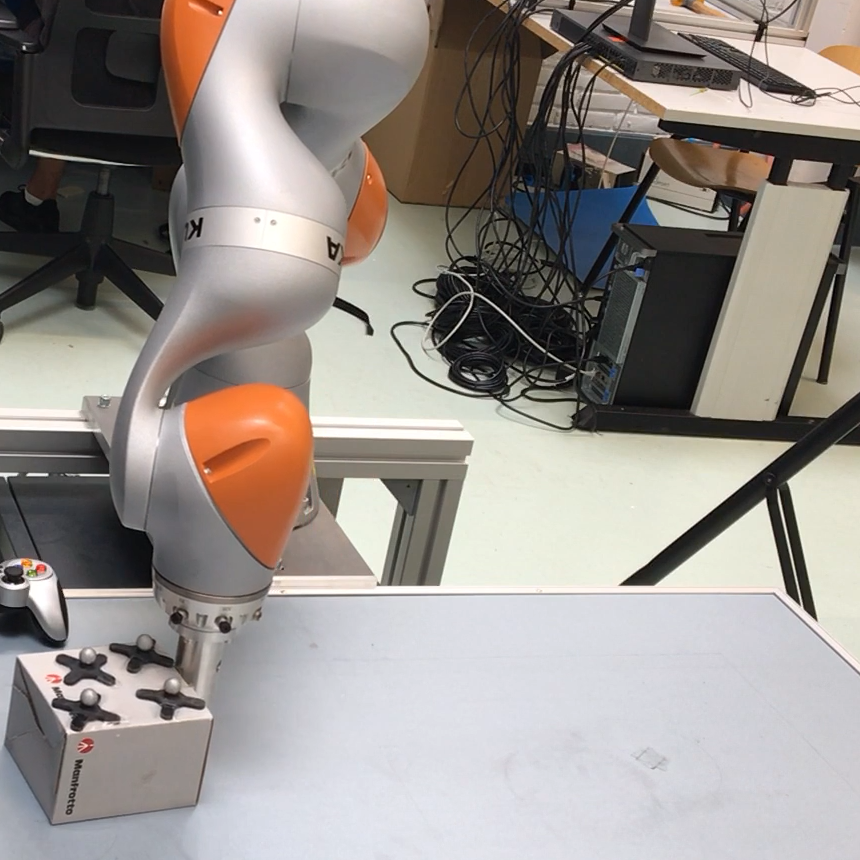
\includegraphics[width=0.19\textwidth]{figures/push5.png}\label{fig:push_pos_2}}
  \caption{Sequence of the task kuka-push-box}.
  \label{fig:sequence-push-box}
\end{figure}







\subsection{Task kuka-park-box}
\label{subsection:Park a box}

The second task also involves pushing a box but this time the sequence of movements is more complex. To achieve the goal the robot has to push in two different axes. First, it has to push the box until a point where it faces the two brown boxes (third frame of Figure \ref{fig:sequence-park-box}). Then, the end effector moves around the corner of the pink box and starts pushing from the other side until the box is fit between the 2 walls. Figure \ref{fig:sequence-park-box} shows the sequence of movements for this task.


 \begin{figure}[H]
  \centering
  \subfloat[1 - Start position]{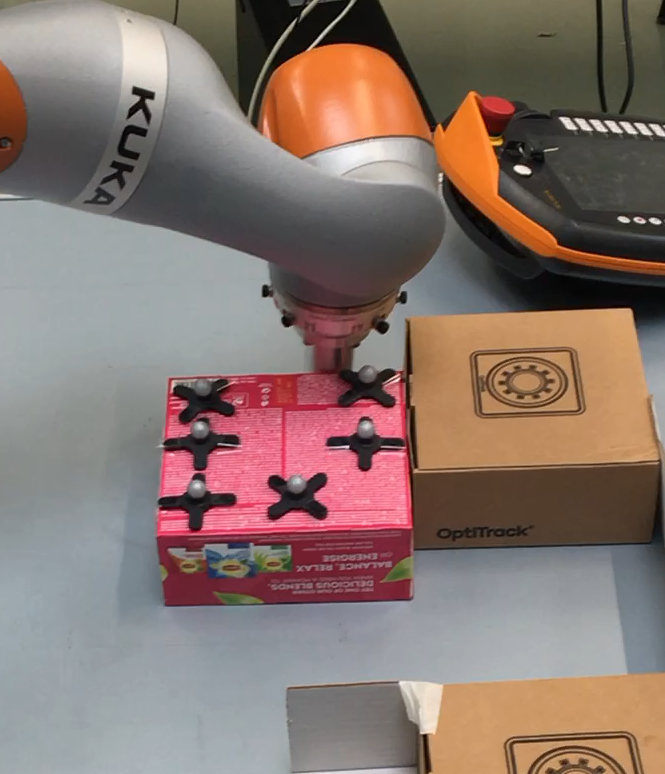
\includegraphics[width=0.16\textwidth]{figures/park0_v2.png}\label{fig:drawer_pos_0}}
   \hfill
  \subfloat[2 - Push box]{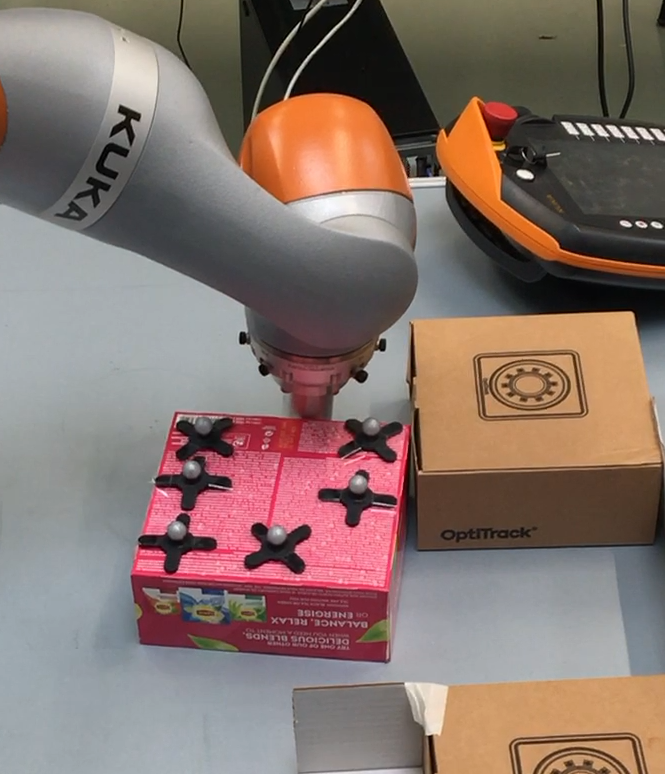
\includegraphics[width=0.16\textwidth]{figures/park1_v2.png}\label{fig:drawer_pos_1}}
   \hfill
  \subfloat[3 - Center box]{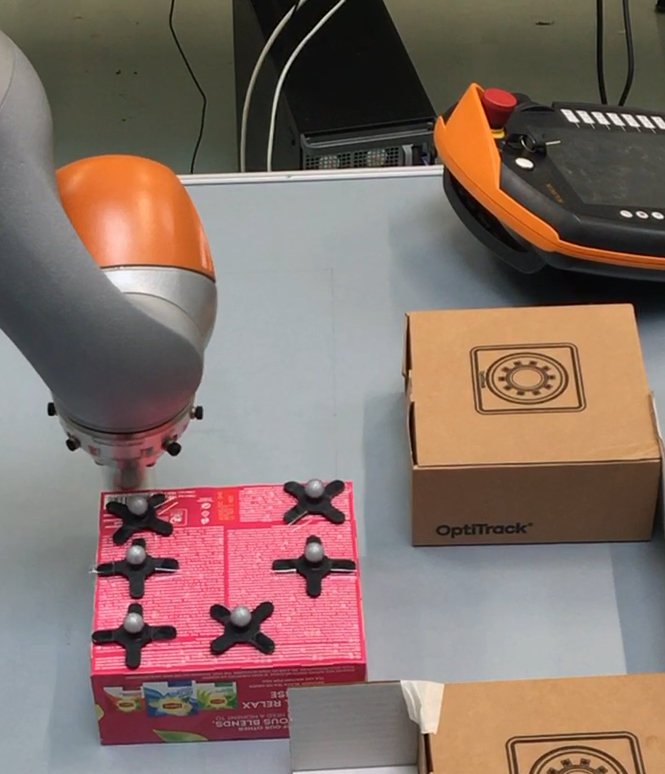
\includegraphics[width=0.16\textwidth]{figures/park3_v2.png}\label{fig:drawer_pos_2}}
   \hfill
  \subfloat[4 - Move around corner]{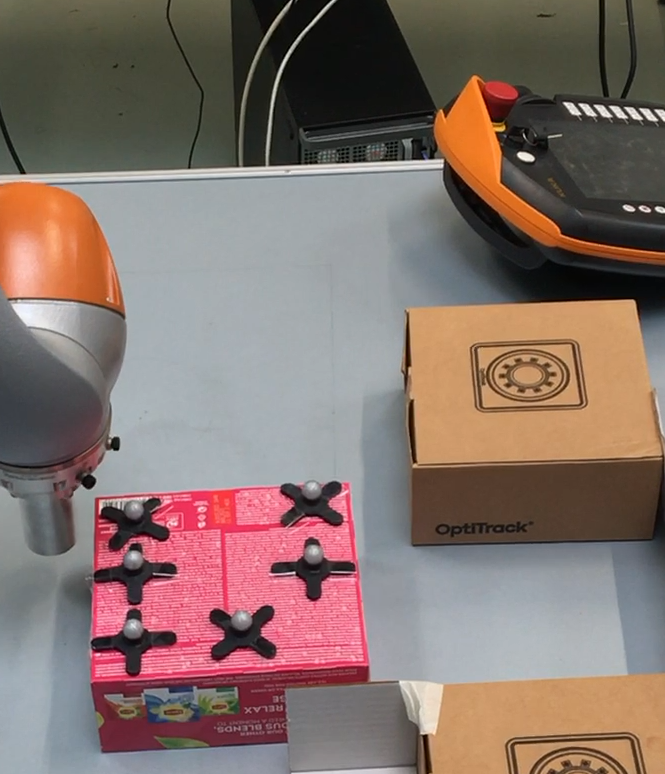
\includegraphics[width=0.16\textwidth]{figures/park4_v2.png}\label{fig:drawer_pos_2}}
   \hfill
  \subfloat[5- Push box between walls]{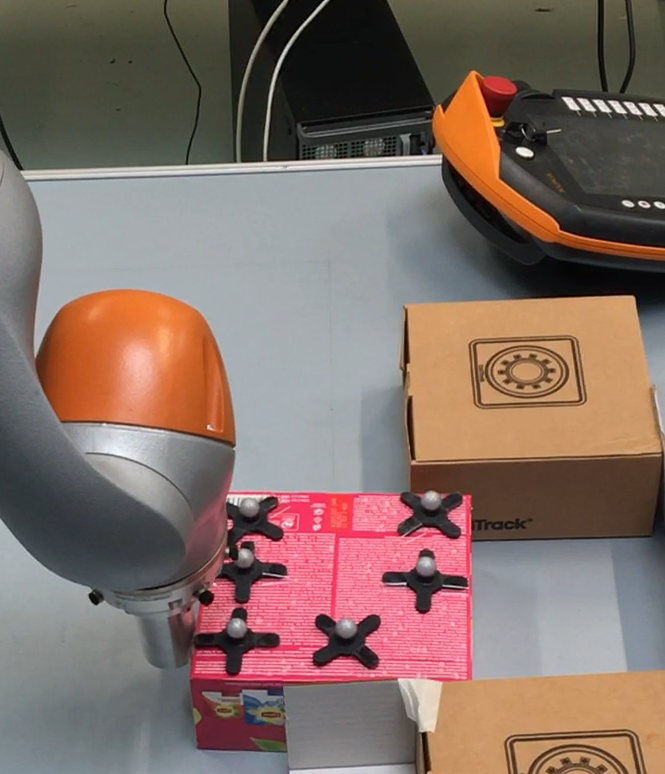
\includegraphics[width=0.16\textwidth]{figures/park5_v2.png}\label{fig:drawer_pos_2}}
   \hfill
  \subfloat[6 - End position]{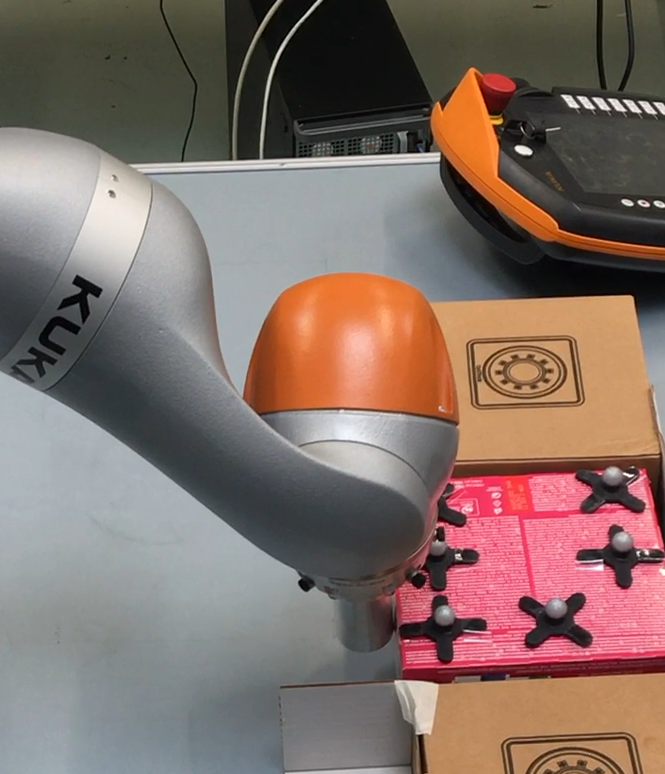
\includegraphics[width=0.16\textwidth]{figures/park6_v2.png}\label{fig:drawer_pos_2}}
  \caption{Sequence of the task kuka-park-box}.
  \label{fig:sequence-park-box}
\end{figure}



